%=========================================
% 	   Implementierung					 =
%=========================================
\chapter{Implementierung}

%=========================================
% 	   Spring							 =
%=========================================
\section{Das Spring-Framework}
\subsection{Warum Spring?}
In dem nun folgenden Abschnitt wird die Frage erläutert warum das Spring Web Framework verwendet 
wurde. Insbesondere welche Alternativen es gab und die jeweiligen Vor- und Nachteile sowie die 
Anforderungen, die an das Web Framework gestellt wurden. \\
Die Projektteilnehmer legten zusammen folgende Anforderungen fest. Zum einen sollte es ein Web-
Framework sein, welches auf Java basiert, da alle Teilnehmer mit dieser Programmiersprache vertraut 
sind. Desweiteren sollte ein standardisiertes Framework eingesetzt werden, da diese getestet sind, 
Code minimieren und somit weniger Fehler und potentielle Fehlerquellen für das Webprojekt bedeuten. 
Weitere Anforderungen waren die Popularität/Zukunftssicherheit, Toolunterstützung, Dokumentation 
und der Support. \\
Nach der Recherchezeit standen folgende Frameworks zur Auswahl:
\begin{itemize}
  \item Spring
  \item Vaadin
  \item Java Server Faces 
  \item Spark
\end{itemize}
\medskip
Im Folgenden werden zu jedem der obigen aufgelisteten Frameworks einige grundlegenden 
Informationen, sowie die Vor- und Nachteile im Bezug auf die oben genannten Anforderungen, für die 
Nutzung der Projektgruppe aufgelistet. 
\begin{description}
	\item [Spring] ist ein auf J2EE basierendes Anwendungsframework und enthält ein eigenes MVC Framework. Es handelt sich dabei um ein Framework welches speziell für die Entwicklung mit Java und JavaEE gedacht ist. Die Vorteile sind, dass es ein quelloffenes Framework ist. Zudem ist es sehr verbreitet, was eine hohe Zukunftssicherheit mit sich bringt. Die Dokumentation und der Support sind durch die häufige Verwendung hervorragend. Bei Spring steht die Entkopplung der Applikationskomponenten im Vordergrund, was nach dem Model-View-Controller Prinzip realisiert wird. Ein Nachteil ist der hohe Einarbeitungsaufwand, da keiner der Projektteilnehmer Erfahrungen mit Web Anwendungen hatte. Dieser Nachteil trifft jedoch auf alle Frameworks zu, insbesondere aber auf das Spring Framework, da es weitere Web Entwicklungstechnologien benutzt, wie Servlets, JavaServer Pages und Faces welche bis dahin auch weitestgehend unbekannt waren.
	\item [Vaadin] ist eine neue Innovative Möglichkeit der Web Entwicklung, welches ebenfalls speziell für die Entwicklung mit Java gedacht ist. Vaadin bietet es eine serverseitige Architektur, was bedeutet, dass der Großteil der Programmlogik auf dem Server läuft. Dadurch hat das Framework eine andere Vorgehensweise als JavaScript Bibliotheken oder auf Browser Plugins basierenden Lösungen. Vaadin ist eine frei verfügbare Software. Der Einstieg in die Web-Entwicklung fällt deutlich leichter als mit dem oben genannten Spring Framework, da einfache Anwendungen intuitiv entwickelt werden können. Es existiert ebenfalls eine umfangreiche Dokumentation und ein guter Support über das Vaadin Forum. Jedoch erfreut sich das Framework zum Zeitpunkt unseres Projekts keiner hohen Popularität, dadurch kann über die Zukunftssicherheit noch keine Prognose getroffen werden. 
	\item [Java Server Faces] ist ein Framework welches in JavaEE bereits integriert ist. Java Server Faces hat eine hohe Popularität. Dadurch besitzt es eine vergleichsweise hohe Zukunftssicherheit. Jedoch ist es wie das Spring Framework für Großprojekte gedacht und verursacht damit bei kleineren Projekten sehr viel Anfangsarbeit (“Oberhead“). Zusätzlich benötigt es Einarbeitungszeit in weitere Basistechnologien, die das Framework nutzt. Die Strukturierung des späteren Projekts (wie auch bei Spring, durch das Model-View-Controller-Konzept realisiert) erhöht die Übersichtlichkeit und ermöglicht eine Wiederverwendung in anderen Projekten.
	\item [Spark] ist ein “kleines“ und einfache zu benutzendes Java Framework für Web Anwendungen. Dabei handelt sich um ein Framework, welches für Echtzeitanalysen d.h. die schnelle Verarbeitung großer Datenmengen gedacht ist. Die Dokumentation ist für die Größe des Frameworks ausreichen. Die Popularität schätzt das Projektteam zum Projektstart relativ gering ein. Jedoch würde es für die Ansprüche im Twitter-Projekt, die geringste Einarbeitungszeit benötigen, da es sehr übersichtlich und intuitiv zu benutzten ist. 
\end{description}

\textit{Auswahl:} Vaadin schied als Innovativsoftware aus, da man keine Prognose für die Zukunftssicherheit machen kann. Somit wäre das Projekt nicht mehr erweiterbar, sollte sich das Framework nicht durchsetzen und vom Markt verschwinden. Spark wurde wegen des zu geringen Supports (Nutzergruppe zu klein) aus der Auswahl gestrichen. Java Server Faces und das Spring Framework befanden sich in der letzten Auswahl. Das Projektteam sah beide als “gleichwertig“ im Bezug auf das gestellte Thema bzw. die gestellte Aufgabe an. Schlussendlich fiel die Entscheidung auf das Spring Framework, da es nicht nur in Web Anwendungen benutzt wird und das Team ihm eine größere Popularität/Zukunftssicherheit zutraut.

\subsection{Spring als Grundlage für das Projekt}

Die konkrete Implementierung ist maßgeblich von der Entscheidung für das Spring Framework
geprägt. Dieses bietet einerseits eine einfache Möglichkeit zum Aufbau einer Servlet-basierten
Webanwendung und andererseits eine flexible Datenbank­schnittstelle. Dadurch ermöglicht es
die Kapselung der eigentlichen Funktionalität in Java Servlets, während die Datenbank und die
Website unabhängig davon aufgebaut werden können. Spring bietet einen modularen Aufbau, somit können
verschiedene Spring Bibliotheken einzeln oder in Kombination verwendet werden. Für dieses Projekt kommen
insbesondere folgende Module zum Einsatz: \\
\begin{itemize}
	\item Die beiden Module \texttt{spring-core} und \texttt{spring-beans} bilden das Fundament des Spring-Frameworks und sind somit unverzichtbar. Sie unterstützen das Konzept der Steuerungsumkehr (\textit{Inversion of Control}) und die entsprechende Erzeugung von \textit{Spring Beans}.
	\item Das \texttt{spring-jdbc} Modul unterstützt JDBC-basierte Anwendungen etwa bei dem Aufbau der Datenbankverbindung, der Konfiguration einer \texttt{Data Source} oder der Erzeugung von \textit{Prepared Statements}.
	\item Das \texttt{spring-webmvc} Modul wird für die Interaktion mit REST-basierten Webservices, sowie für die Implementierung einer \acs{MVC}-Architektur benötigt.
	\item Das \texttt{spring-security} Paket stellt ein eigenständiges Spring Sub-Projekt dar und kann wiederum in diverse Module unterteilt werden. Es bietet in erster Linie verschiedene Methoden zur Authentifizierung und Autorisierung in J2EE-Anwendungen.
\end{itemize}

\subsubsection*{Spring Beans}
Spring grenzt sich von anderen \textit{Java Enterprise} Frameworks insofern ab, als dass keine standardisierten Komponenten, wie etwa \acs{EJBs}, verwendet werden, sondern vielmehr eine lose Kopplung von \acs{POJO}s\footnote{Ein \ac{POJO} ist in diesem Kontext ein Objekt, das nicht mittels Oberklassen oder Interfaces spezialisiert ist. Es stellt somit die einfachste Form eines Objektes im Sinne der Objektorientierung dar.} fokussiert wird. In diesem Zusammehang bezeichnet man die Objekte einer auf Spring basierten Anwendung auch als \textit{Spring Beans}. Jede \textit{Spring Bean} Instanz definiert sich über konfigurationsspezifische Metadaten, die entweder explizit (mittels Java oder XML) oder implizit (mittels \textit{Autowiring}) festgelegt werden. In Tabelle \ref{tab:spring_config} sind die wichtigsten Eigenschaften einer \textit{Spring Bean} in Bezug auf Konstruktion, Lebenszyklus und Abhängigkeiten aufgelistet. 

\begin{table}[!ht]
\caption[Konfiguration einer \textit{Spring Bean}, in Anlehnung an \cite{tuto:beans}]{Konfiguration einer \textit{Spring Bean} \cite{tuto:beans}}
\label{tab:spring_config} 
  \begin{tabular}{p{4.8cm}p{9.4cm}}
    \toprule 
    \textbf{Eigenschaft} & \textbf{Beschreibung}  \\
    \hline 
    \texttt{class} & Legt die Klasse einer \textit{Bean} fest. \\
    \texttt{name / id} & Indentifiziert jede \textit{Spring Bean} eindeutig. \\
    \texttt{scope} & Spezifiziert den Kompetenzbereich einer \textit{Bean}. Unterschieden wird hierbei zwischen Singleton, Prototyp, Request und Session. \\
     \texttt{constructor-arg} & Definiert die, bei einer Konstruktor-basierten \textit{Dependency Injection} auftretenden Abhängigkeiten als Konstruktorargumente \\
      \texttt{properties} & Definiert die, bei einer \texttt{Setter}-basierten \textit{Dependency Injection} auftretenden Abhängigkeiten als Methodenparameter \\
      \texttt{autowiring mode} & Aktiviert die Konfiguration von Abhängigkeiten mittels \textit{Autowiring}. \\
      \texttt{lazy-initialization mode} & Impliziert eine Erstellung der Instanz nach tatsächlichem Bedarf, im Gegensatz zu einer Konstruktion beim Starten des Programms. \\
      \texttt{initialization method} & Definiert eine Methode, welche unmittelbar nach der Initialisierung einer \textit{Bean} aufgerufen wird. \\
      \texttt{destruction method} & Definiert eine Methode, welche unmittelbar nach der Destruktion einer \textit{Bean} aufgerufen wird. \\
   	\bottomrule
  \end{tabular}
\end{table}

\newpage
Ein Anwendung für die explizite Angabe von Konfigurationsdetails via XML, findet sich am Beispiel dieses Projektes in der Definition des \texttt{ViewResolvers}, welcher in den Abschnitten \ref{subsec:spring_mvc} und \ref{sec:frontend} genauer betrachtet wird:
\smallskip
\begin{lstlisting}[style=XML]
<bean id="ViewResolver"
		class="org.springframework.web.servlet.view.InternalResourceViewResolver">
		<property name="prefix" value="/WEB-INF/jsps/"></property>
		<property name="suffix" value=".jsp"></property>
</bean>
\end{lstlisting} 
\medskip 

\subsubsection*{Inversion of Control}
Einhergehend mit der losen Kopplung von \textit{Spring Beans}, werden deren Abhängigkeiten zu anderen Klassen zentral verwaltet. Man spricht hier von Steuerungsumkehr oder auch \textit{Inversion of Control} (\acs{IoC}). Darunter versteht man insbesondere die automatische Erstellung und
	Referenzierung von Objekten durch eine gemeinsame \texttt{ApplicationContext} Instanz. Abbildung \ref{fig:spring_context} veranschaulicht dieses Konzept.	
\begin{figure}[!h]
    \centering
    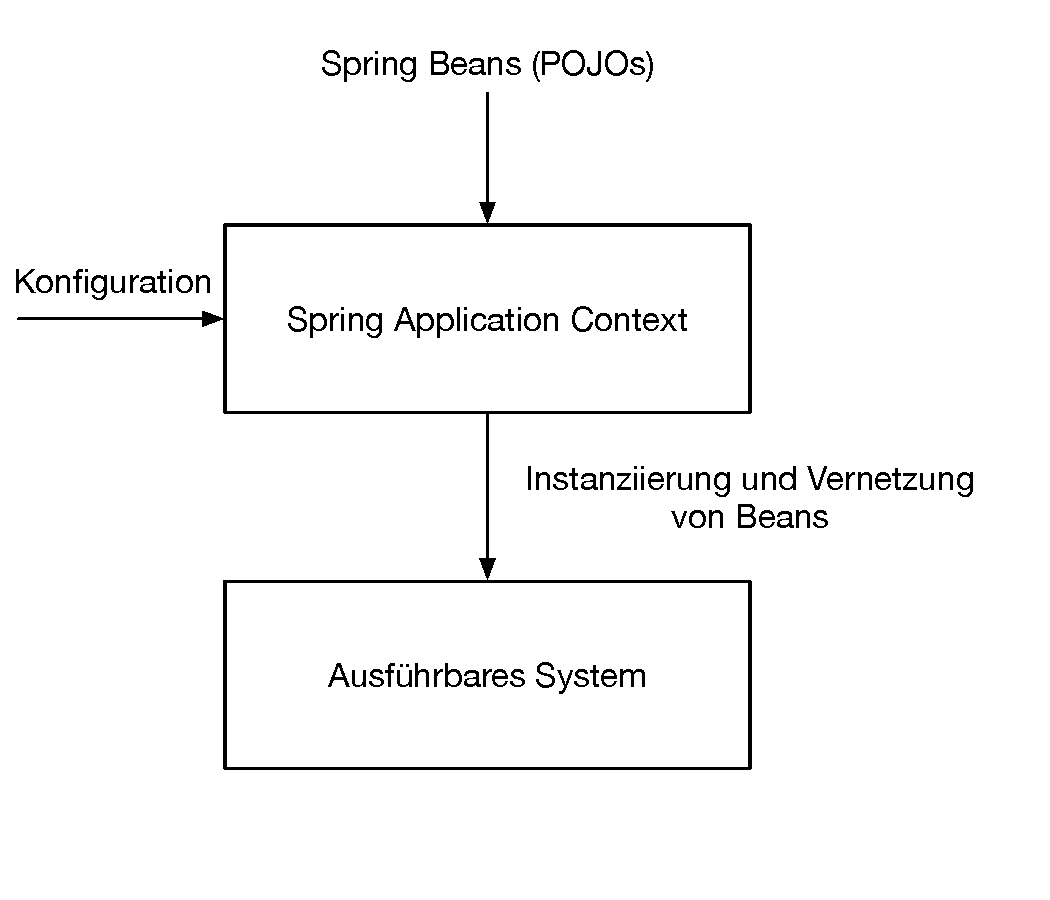
\includegraphics[width=0.85\textwidth]{Graphics/spring_context}
    \caption[Grundprinzip einer Springanwendung, in Anlehnung an: \cite{tuto:ioc}]{Grundprinzip einer Springanwendung \cite{tuto:ioc}}
   \label{fig:spring_context}
\end{figure}
%
Auf diese Art und Weise können Abhängigkeiten einer \textit{Bean} unter Berücksichtigung der Konfigurationsdaten während der Laufzeit erzeugt werden. Dies wird im Allgemeinen auch als \textit{Dependency Injection} bezeichnet. Man unterscheidet dabei zwischen einer Injizierung der Abhängigkeiten mittels Konstruktor (\textit{Constructor Injection}) oder mittels einer eigens dafür vorgesehenen Methode (\textit{Setter Injection}). Wie bereits erwähnt, kann die Konifguration der Beziehungen zwischen Beans automatisch erfolgen.
\newpage
\subsubsection*{Autowiring}
\textit{Autowiring} bezeichnet im Wesentlichen die implizite Verknüpfung von \textit{Spring Beans} durch das Spring-Framework selbst. Ziel dabei ist es den Konfigurationsaufwand zu minimieren. Um dies zu erreichen, muss der \texttt{ApplicationContext} Beans automatisch finden und als solche erkennen können. Dieser Prozess ist als \textit{Component Scanning} in das Framework integriert, muss aber unter Angabe des Packages, in dem sich die zugehörigen Klassen befinden, explizit aktiviert werden:
\medskip
\begin{lstlisting}[style=XML]
<context:component-scan base-package="de.htwsaar.db">
			</context:component-scan>
<mvc:annotation-driven></mvc:annotation-driven>
\end{lstlisting} 
\medskip 
Ebenso müssen Klassen, welche als \textit{Bean} instanziiert werden sollen, mittels \textit{Annotation} als solche gekennzeichnet werden. Das \textit{spring-webmvc} Modul unterstützt hierbei verschiedene Annotationen, wie etwa \texttt{@Controller}, \texttt{@Service} oder \texttt{@Component}, welche die jeweilge Schicht der Architektur widerspiegeln. Darüber hinaus kann die Annotation durch einen Namen qualifiziert werden, sodass später eine eindeutige Zuordnung möglich ist.
\medskip
\begin{lstlisting}[style=Java]
@Component("keywordDao")
public class KeywordDao { 
	...
}

...

@Service
public class KeywordService {

	private KeywordDao keywordDao;

	@Autowired
	public KeywordService(KeywordDao keywordDao) {
		this.keywordDao = keywordDao;
	}
...
}
\end{lstlisting} 
\medskip 
Im obigen Beispiel veranlasst die Annotation \texttt{@Autowired} nun ein Scannen der Komponenten. Wird hierbei die entsprechende Bean gefunden, kann diese instanziiert und referenziert werden. 
 
